\documentclass{amsart}
\usepackage{amssymb}
\usepackage{graphicx}
\usepackage[hidelinks]{hyperref}

\newtheorem{theorem}{Theorem}[section]
\newtheorem{lemma}[theorem]{Lemma}
\newtheorem{proposition}[theorem]{Proposition}
\newtheorem{corollary}[theorem]{Corollary}
\newtheorem{conjecture}{Conjecture}
\renewcommand{\theconjecture}{\Alph{conjecture}}
\theoremstyle{definition}
\newtheorem{definition}[theorem]{Definition}
\theoremstyle{remark}
\newtheorem{remark}[theorem]{Remark}

\numberwithin{equation}{section}

\newcommand{\Z}{\mathbb{Z}}
\newcommand{\F}{\mathbb{F}}
\newcommand{\gp}[1]{[#1]}
\newcommand{\zenodoID}{10.5281/zenodo.23398805}
\newcommand{\preprintURL}{https://github.com/creelie/refactored-waddle/blob/main/preprintGolombWelchRadiusThree/GolombWelchRadiusThree.pdf}

\begin{document}

\title[Lattice tilings by Lee balls of radius three]{No lattice tiling of $\mathbb{Z}^{35}$ or $\mathbb{Z}^{805}$ by Lee balls of radius three}

\author[D. Bhattacharjee]{Deep Bhattacharjee}
\address{Formerly, Electro-Gravitational Space Propulsion Laboratory (EGSPL),\newline Bhubaneswar, Odisha 751030, India; Formerly, University of Calcutta, Senate House,\newline 87/1 College Street, Kolkata 700073, West Bengal, India}
\email{itsdeep@live.com}
\email{d.bhattacharjee@erl-forschung.de}
\urladdr{https://orcid.org/0000-0003-0466-750X}
\thanks{Corresponding author: Deep Bhattacharjee.}

\author[U. Bhattacharya]{Ushashi Bhattacharya}
\address{Formerly, National Taiwan University, Taipei 106319, Taiwan}
\email{rai.bhattacharya.in@gmail.com}
\urladdr{https://orcid.org/0009-0002-2254-3914}

\subjclass[2020]{Primary 52C22; Secondary 05B45, 94B25, 05C25}
\keywords{Golomb--Welch conjecture, Lee metric, perfect code, lattice tiling, group ring}

\begin{abstract}
We prove that there is no lattice tiling of $\mathbb{Z}^{35}$ or of $\mathbb{Z}^{805}$ by Lee balls of radius three. These were the only cases left open by Xiao and Zhou among the Lee balls of dimension at least three and radius at least two with fewer than $2^{30}$ points, so the lattice Golomb--Welch conjecture holds for all of them.
\end{abstract}

\maketitle

\section{Introduction}

For integers $n\ge1$ and $r\ge0$ the Lee ball of radius $r$ in $\Z^n$ is
\[
B^n(r)=\{a\in\Z^n:\ |a_1|+\dots+|a_n|\le r\}.
\]
A \emph{tiling} of $\Z^n$ by $B^n(r)$ is a set $T\subset\Z^n$ such that the translates $t+B^n(r)$ with $t\in T$ partition $\Z^n$, and it is a \emph{lattice tiling} if $T$ is a subgroup of $\Z^n$. Such tilings exist when $n\le2$ and when $r=1$.\footnote{A lattice tiling by $B^n(r)$ is a lattice packing of translates of $B^n(r)$ with density one, so the question is the extreme case of the lattice packing problem for the Lee ball, the $\ell^1$ counterpart of the Euclidean ball. For the Euclidean problem in dimensions four and seven, where the densest lattices are $D_4$ and $E_7$, see \cite{BBB26a,BBB26b}; there the obstacle is to compare every packing with one lattice, whereas here it is to show that a single lattice cannot exist.} Golomb and Welch~\cite{GW} conjectured that these are the only cases.

\begin{conjecture}[Golomb--Welch]\label{conj:gw}
For $n\ge3$ and $r\ge2$ there is no tiling of $\Z^n$ by $B^n(r)$.
\end{conjecture}

The conjecture is open, and so is its lattice form, in which only lattice tilings are considered. It holds for $3\le n\le5$ \cite{GMP,Hor09} and for radii that are large compared with the dimension \cite{Post,HK}; the lattice form holds for radius two in every dimension~\cite{LZ}. We refer to the survey of Horak and Kim~\cite{HK} for the history. A lattice tiling is the same thing as a perfect code in a finite abelian group~\cite{HA}, and in this form many further dimensions have been excluded for small radii by the polynomial method and by group-ring equations \cite{Kim,ZG17,ZZ,Qur,ZG24}. Xiao and Zhou~\cite{XZ} recently combined all these criteria with new ones and applied them to every pair $(n,r)$ with $n\ge3$, $r\ge2$ and $|B^n(r)|<2^{30}$. Of the $1358$ such pairs they excluded $1356$, and the two that remained are $(n,r)=(35,3)$ and $(805,3)$ \cite[Theorem~5.1]{XZ}. We settle both.

\begin{theorem}\label{thm:main}
There is no lattice tiling of $\Z^{35}$ by $B^{35}(3)$, and there is no lattice tiling of $\Z^{805}$ by $B^{805}(3)$.
\end{theorem}

\begin{corollary}\label{cor:main}
If $n\ge3$, $r\ge2$ and $|B^n(r)|<2^{30}$, then $\Z^n$ has no lattice tiling by $B^n(r)$.
\end{corollary}

\begin{proof}
This is Theorem~\ref{thm:main} together with \cite[Theorem~5.1]{XZ}.
\end{proof}

The balls in question have
\[
|B^{35}(3)|=59711=29^2\cdot71,\qquad |B^{805}(3)|=696845031=3\cdot29^2\cdot179\cdot1543.
\]
Neither number is prime, so the theorem of Szegedy~\cite{Sze}, which turns the nonexistence of lattice tilings into the nonexistence of all tilings when $|B^n(r)|$ is prime, does not apply, and Theorem~\ref{thm:main} says nothing about tilings that are not lattice tilings. In the language of the degree--diameter problem~\cite{DF}, Theorem~\ref{thm:main} says that no abelian group of order $59711$ is generated by $35$ elements in such a way that each of its elements is a sum of at most three of these generators and their negatives, and likewise for order $696845031$ and $805$ generators; in other words the abelian Cayley--Moore bound is not attained in degree $70$ or in degree $1610$ at diameter three (compare \cite[Section~1]{XZ}).\footnote{The statement concerns the word metric of the Cayley graph of $G$ with respect to $\pm g_1,\dots,\pm g_n$: every element has word length at most three, and the lattice tiling asks that the shortest word be unique. This is the opposite extreme from the word metrics of hyperbolic groups, where the Cayley graph is negatively curved at large scale \cite{Bha22}; in an abelian group the ball of radius three is as small as it can be, and the tiling asks it to be exactly as large as $B^n(3)$.}

\subsection*{The method}
A lattice tiling of $\Z^n$ by $B^n(3)$ gives a finite abelian group $G$ of order $|B^n(3)|$ and elements $g_1,\dots,g_n$ such that $a\mapsto\sum_ja_jg_j$ maps $B^n(3)$ bijectively onto $G$ (Lemma~\ref{lem:reduction}). Summing a character over the ball gives a cubic identity in a group ring (Proposition~\ref{prop:ball}), and projecting $G$ onto $\Z/p$ for a prime $p$ dividing $|G|$ turns it into conditions on the images of the $g_j$. This is the setting of~\cite{ZZ,XZ}, and two features of the present cases defeat the projections used so far.

For $n=805$ the conditions modulo $p=29$ leave a very large number of possible distributions of the images, whose examination Xiao and Zhou estimated would take about two months of exhaustive search \cite[Example~5.13]{XZ}. We read off the coefficient of the identity element modulo $29^2$ instead; it excludes all of them by one congruence (Section~\ref{sec:805}).

For $n=35$ Xiao and Zhou found, for each of the two primes $71$ and $29$, a distribution of the images that satisfies every condition coming from that prime alone \cite[Example~5.14]{XZ}. We project onto $\Z/71\times\Z/29$ at once, through a character with values in the dual numbers over the group ring $\F_{71}[\Z/29]$. The first-order part of the identity couples the two distributions and leads to a circulant linear system over $\F_{71}$ whose only solution is zero (Section~\ref{sec:35}). Figure~\ref{fig:roadmap} shows the order of the argument.

\begin{figure}[ht]
\centering
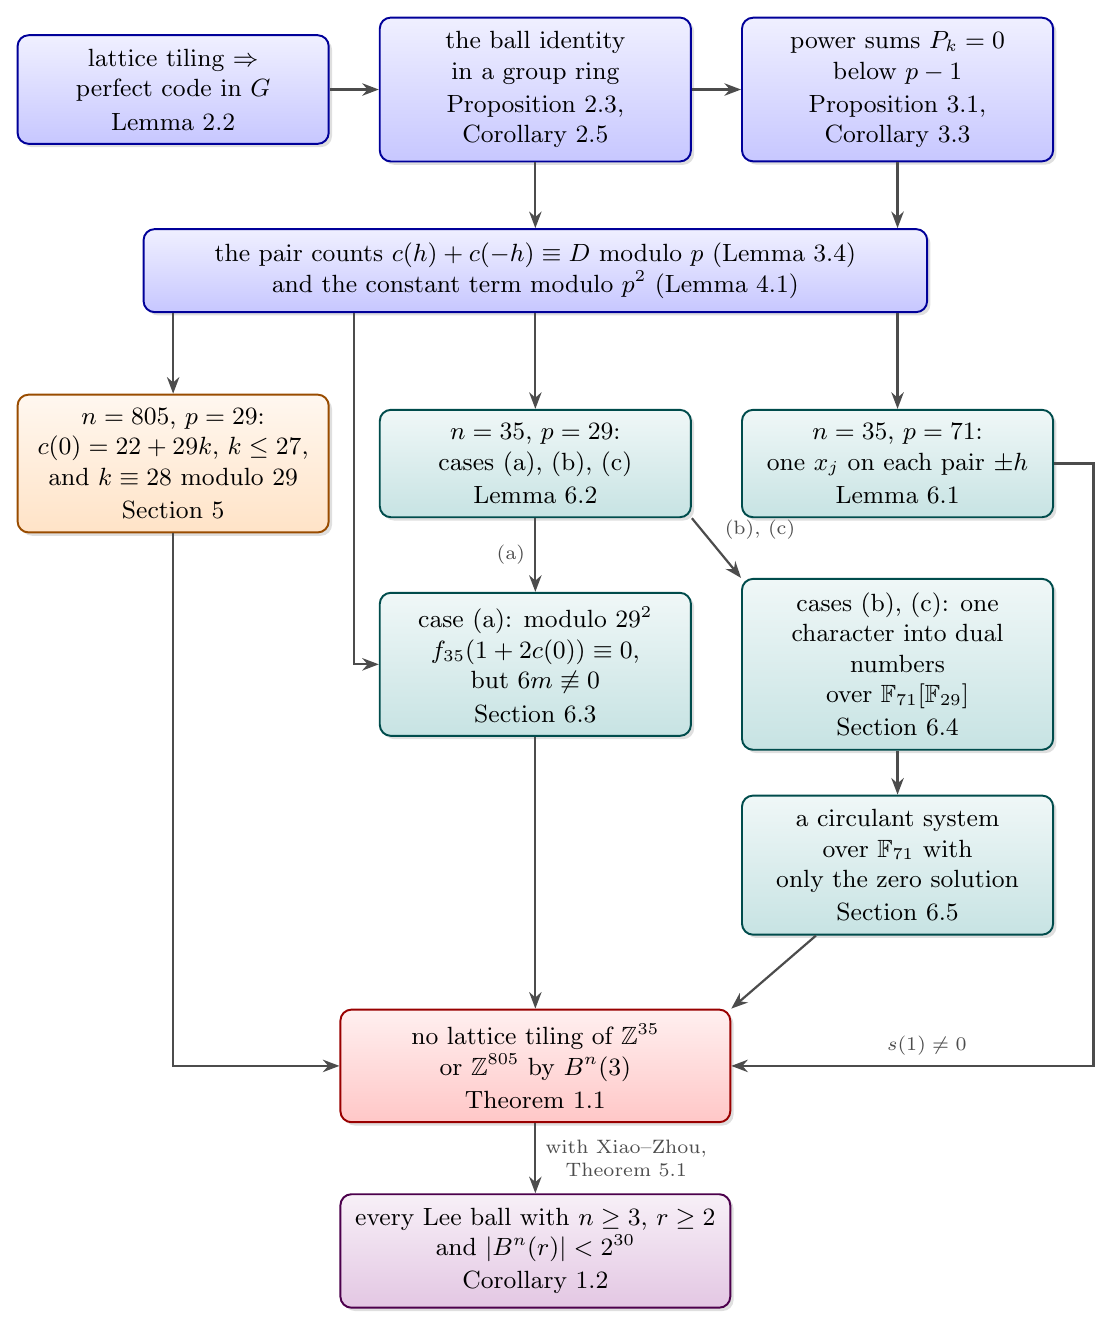
\includegraphics[width=0.95\textwidth]{figures/fig_roadmap.png}
\caption{The order of the proof. Arrows point from a result to the results that use it.}
\label{fig:roadmap}
\end{figure}

Theorem~\ref{thm:main}, with every step of Sections~\ref{sec:codes}--\ref{sec:35}, has been formalized in the Lean~4 proof assistant (Section~\ref{sec:lean}).

\section{Perfect codes and the ball identity}\label{sec:codes}

All groups in this paper are abelian and written additively, except the groups of units of rings. For $a\in\Z^n$ we write $|a|=|a_1|+\dots+|a_n|$, and $B^n=B^n(3)$.

\begin{definition}
Let $G$ be a finite group and $g=(g_1,\dots,g_n)\in G^n$. Put $\varphi_g(a)=\sum_ja_jg_j$ for $a\in\Z^n$. We call $g$ a \emph{perfect code} in $G$ if $\varphi_g$ maps $B^n$ bijectively onto $G$.
\end{definition}

\begin{lemma}\label{lem:reduction}
Let $L\subseteq\Z^n$ be a subgroup such that the translates $l+B^n$, $l\in L$, partition $\Z^n$. Let $e_1,\dots,e_n$ be the unit vectors. Then $G=\Z^n/L$ is finite, $(e_1+L,\dots,e_n+L)$ is a perfect code in $G$, and $|G|=|B^n|$.
\end{lemma}

\begin{proof}
Here $\varphi_g(a)=a+L$. Every $x\in\Z^n$ lies in a translate $l+B^n$ with $l\in L$, and then $a=x-l\in B^n$ satisfies $\varphi_g(a)=x+L$; so $\varphi_g$ maps $B^n$ onto $G$, and $G$ is finite. If $a,b\in B^n$ and $a-b\in L$, the point $a$ lies in $0+B^n$ and in $(a-b)+B^n$, because $a-(a-b)=b\in B^n$. The translates are disjoint, so $a-b=0$. Hence $\varphi_g$ is injective on $B^n$, and $|G|=|B^n|$.
\end{proof}

Figure~\ref{fig:ball} shows the ball $B^3(3)$, the tile of the three-dimensional case.

\begin{figure}[ht]
\centering
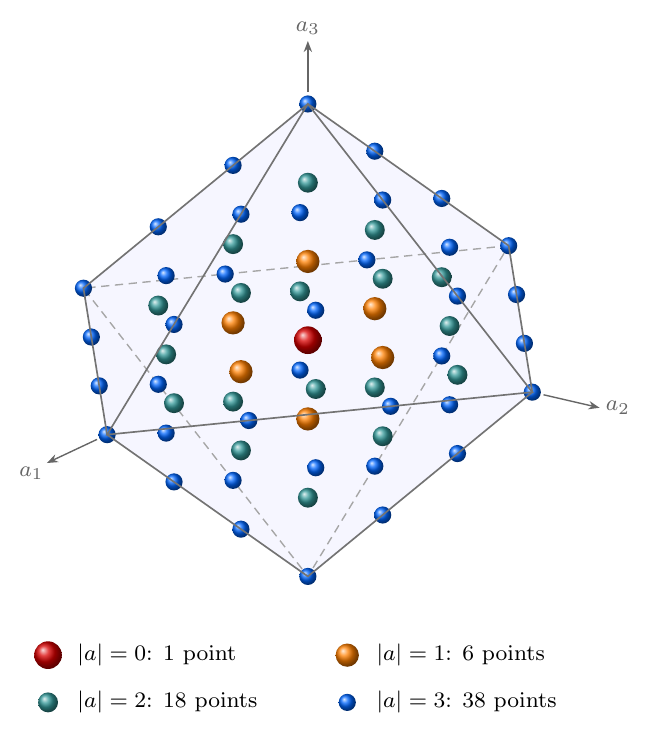
\includegraphics[width=0.52\textwidth]{figures/fig_ball.png}
\caption{The Lee ball $B^3(3)$: the $63$ points of $\Z^3$ in the octahedron $|a_1|+|a_2|+|a_3|\le3$, shaded by $|a|$. A lattice tiling translates it by the points of a subgroup $L$; the quotient $\Z^3/L$ then has one element for each point of the ball.}
\label{fig:ball}
\end{figure}

The next identity is the source of all the conditions used below. Let $f_n$ be the polynomial
\[
f_n(X)=X^3+3X^2+2X-6nX=X(X+1)(X+2)-6nX.
\]

\begin{proposition}\label{prop:ball}
Let $R$ be a commutative ring, $\Gamma$ a group, $\chi\colon\Gamma\to R^\times$ a homomorphism, and $z_1,\dots,z_n\in\Gamma$. For $i=1,2,3$ put $T_i=1+\sum_j\bigl(\chi(iz_j)+\chi(-iz_j)\bigr)$. Then
\begin{equation}\label{eq:ball}
6\sum_{a\in B^n}\chi\Bigl(\sum_ja_jz_j\Bigr)=T_1^3+3T_1T_2+2T_3-6nT_1.
\end{equation}
\end{proposition}

\begin{proof}
Put $u_j=\chi(z_j)$ and $v_j=\chi(-z_j)$, so that $u_jv_j=1$ and $\chi(\sum_ja_jz_j)=\prod_ju_j^{a_j}$, where $u_j^{-1}=v_j$. Consider multisets of the letters $u_1,\dots,u_n$ and $v_1,\dots,v_n$, and say that a multiset contains a \emph{pair} if it contains both $u_j$ and $v_j$ for some $j$. A multiset $M$ of size $k$ without a pair corresponds to the point $a\in\Z^n$ with $a_j$ equal to the multiplicity of $u_j$ minus that of $v_j$; this is a bijection onto the points with $|a|=k$, and the product of the elements of $M$ is $\prod_ju_j^{a_j}$.

Let $h_k$ be the sum, over all multisets $M$ of size $k$, of the product of the elements of $M$, and let $p_i=\sum_j(u_j^i+v_j^i)$. The multisets of size $2$ with a pair are the $n$ multisets $\{u_j,v_j\}$, each with product $1$. A multiset of size $3$ with a pair is $\{u_j,v_j,w\}$ for one index $j$ and one letter $w$, these are distinct for distinct $(j,w)$, and the product is $w$. Hence
\[
\sum_{a\in B^n}\prod_ju_j^{a_j}=1+p_1+(h_2-n)+(h_3-np_1).
\]
Newton's identities give $2h_2=p_1^2+p_2$ and $6h_3=p_1^3+3p_1p_2+2p_3$ in the polynomial ring over $\Z$ in the $2n$ letters, hence in $R$. Six times the right side above is therefore
\[
6+6p_1+3p_1^2+3p_2-6n+p_1^3+3p_1p_2+2p_3-6np_1,
\]
which is $T_1^3+3T_1T_2+2T_3-6nT_1$ for $T_i=1+p_i$.
\end{proof}

With $\Gamma$ trivial, \eqref{eq:ball} reads $6|B^n|=f_n(2n+1)$. For instance $|B^{35}|=f_{35}(71)/6=59711$ and $|B^{805}|=f_{805}(1611)/6=696845031$.

\begin{lemma}\label{lem:uniform}
Let $g$ be a perfect code in $G$, let $\psi\colon G\to\Gamma$ be a surjective homomorphism onto a finite group $\Gamma$, and let $F\colon\Gamma\to M$ be a map to a group $M$. Then
\[
\sum_{a\in B^n}F\Bigl(\sum_ja_j\psi(g_j)\Bigr)=\frac{|G|}{|\Gamma|}\sum_{\gamma\in\Gamma}F(\gamma).
\]
\end{lemma}

\begin{proof}
The argument of $F$ is $\psi(\varphi_g(a))$, and $\varphi_g$ maps $B^n$ bijectively onto $G$, so the left side is $\sum_{x\in G}F(\psi(x))$. Each fibre of $\psi$ has $|G|/|\Gamma|$ elements.
\end{proof}

For a commutative ring $k$ and a finite group $\Gamma$ we write $k[\Gamma]$ for the group ring, with basis elements $\gp{\gamma}$, $\gamma\in\Gamma$, multiplied by $\gp{\gamma}\gp{\gamma'}=\gp{\gamma+\gamma'}$. Its unit element is $\gp0$, and we write $S_\Gamma=\sum_{\gamma\in\Gamma}\gp{\gamma}$. For $F\in k[\Gamma]$ we write $F(\gamma)$ for the coefficient of $\gp{\gamma}$.

\begin{corollary}\label{cor:projected}
Let $g$ be a perfect code in $G$, let $\psi\colon G\to\Gamma$ be surjective, and put $x_j=\psi(g_j)$.
\begin{enumerate}
\item If $\chi\colon\Gamma\to R^\times$ is a homomorphism into the units of a commutative ring and $T_i=1+\sum_j(\chi(ix_j)+\chi(-ix_j))$, then
\begin{equation}\label{eq:chi}
6\,\frac{|G|}{|\Gamma|}\sum_{\gamma\in\Gamma}\chi(\gamma)=T_1^3+3T_1T_2+2T_3-6nT_1.
\end{equation}
\item In $k[\Gamma]$, with $T_i=\gp0+\sum_j(\gp{ix_j}+\gp{-ix_j})$,
\begin{equation}\label{eq:groupring}
6\,\frac{|G|}{|\Gamma|}\,S_\Gamma=T_1^3+3T_1T_2+2T_3-6nT_1.
\end{equation}
\end{enumerate}
\end{corollary}

\begin{proof}
Apply Proposition~\ref{prop:ball} with $z_j=x_j$ and then Lemma~\ref{lem:uniform} with $F=\chi$. Part~(2) is the case $R=k[\Gamma]$, $\chi(\gamma)=\gp{\gamma}$.
\end{proof}

\begin{lemma}\label{lem:surj}
If a prime $p$ divides $|G|$, there is a surjective homomorphism $G\to\Z/p$.
\end{lemma}

\begin{proof}
Write $G$ as a direct sum of cyclic groups of prime power order. Since $p$ divides $|G|$, one summand is $\Z/p^e$ with $e\ge1$; project onto it and reduce modulo $p$.
\end{proof}

\section{Power sums modulo a prime}\label{sec:moments}

Throughout this section $g$ is a perfect code in a group $G$ with $|G|=|B^n|$, $p$ is a prime dividing $|G|$, and $\psi\colon G\to\F_p=\Z/p$ is surjective. We put
\begin{gather*}
x_j=\psi(g_j),\qquad m=\frac{|G|}{p},\qquad c(h)=\#\{j:\ x_j=h\}\ \ (h\in\F_p),\\
P_k=\sum_j\bigl(x_j^k+(-x_j)^k\bigr)\in\F_p,
\end{gather*}
with $0^0=1$. For odd $k$ the two terms of each summand cancel, so $P_k=0$. For $F\in\F_p[\F_p]$ and $k\ge0$ we define the moment $M_k(F)=\sum_{h\in\F_p}F(h)h^k\in\F_p$. Expanding $(h+h')^k$ gives
\begin{equation}\label{eq:leibniz}
M_k(FF')=\sum_{i=0}^{k}\binom{k}{i}M_i(F)M_{k-i}(F').
\end{equation}
For $T_i=\gp0+\sum_j(\gp{ix_j}+\gp{-ix_j})$ we have $M_0(T_i)=2n+1$ and $M_k(T_i)=i^kP_k$ for $k\ge1$.

\begin{proposition}\label{prop:moment}
Let $v\ge1$, and suppose that $P_k=0$ for $1\le k<v$. Then $\kappa_n(v)\,P_v=6m\sum_{h\in\F_p}h^v$, where
\[
\kappa_n(v)=3(2n+1)^2+3(2n+1)(1+2^v)+2\cdot3^v-6n.
\]
\end{proposition}

\begin{proof}
Call $F$ \emph{flat} if $M_k(F)=0$ for $1\le k<v$. By~\eqref{eq:leibniz} a product of flat elements is flat, and for flat $F,F'$ we have $M_v(FF')=M_0(F)M_v(F')+M_v(F)M_0(F')$. The $T_i$ are flat by hypothesis, so
\begin{gather*}
M_v(T_1^3)=3(2n+1)^2P_v,\qquad M_v(T_1T_2)=(2n+1)(1+2^v)P_v,\\
M_v(T_3)=3^vP_v,\qquad M_v(T_1)=P_v.
\end{gather*}
Apply $M_v$ to~\eqref{eq:groupring} with $k=\Gamma=\F_p$; the left side becomes $6m\sum_hh^v$.
\end{proof}

\begin{lemma}\label{lem:powersums}
$\sum_{h\in\F_p}h^v=0$ for $1\le v<p-1$, and $\sum_{h\in\F_p}h^{p-1}=-1$.
\end{lemma}

\begin{proof}
If $1\le v<p-1$, a generator $u$ of the cyclic group $\F_p^\times$ has $u^v\ne1$, and $\sum_hh^v=\sum_h(uh)^v=u^v\sum_hh^v$. If $v=p-1$, then $h^v=1$ for $h\ne0$.
\end{proof}

\begin{corollary}\label{cor:flat}
Let $2\le L\le p-1$, and suppose that $\kappa_n(v)\ne0$ in $\F_p$ for every even $v$ with $2\le v<L$. Then $P_k=0$ for $1\le k<L$.
\end{corollary}

\begin{proof}
By induction on $k$. For odd $k$ we have seen that $P_k=0$. For even $k<L$, Proposition~\ref{prop:moment} with $v=k$ and Lemma~\ref{lem:powersums} give $\kappa_n(k)P_k=0$.
\end{proof}

When all power sums below $p-1$ vanish, the distribution of the $x_j$ is almost determined.

\begin{lemma}\label{lem:counts}
Suppose that $P_k=0$ for $1\le k<p-1$, and let $D\in\{0,\dots,p-1\}$ be the integer with $D\equiv-P_{p-1}\pmod p$.
\begin{enumerate}
\item $c(h)+c(-h)\equiv D\pmod p$ for every $h\ne0$, and $2c(0)\equiv2n+D\pmod p$.
\item $(p-1)D+2c(0)\le2n$, and if equality holds, then $c(h)+c(-h)=D$ for every $h\ne0$.
\end{enumerate}
\end{lemma}

\begin{proof}
(1) Let $F=T_1-(2n+1)\gp0$, so that $F(h)=c(h)+c(-h)-2n\,\delta_{h,0}$, $M_0(F)=0$ and $M_k(F)=P_k$ for $k\ge1$. Fix $h\in\F_p$. Expanding $(h'-h)^{p-1}$ by the binomial theorem gives
\[
\sum_{h'}F(h')(h'-h)^{p-1}=\sum_{i=0}^{p-1}\binom{p-1}{i}(-h)^{p-1-i}M_i(F)=M_{p-1}(F)=P_{p-1}.
\]
On the other hand $(h'-h)^{p-1}$ is $1$ for $h'\ne h$ and $0$ for $h'=h$, so the left side is $M_0(F)-F(h)=-F(h)$. Thus $F(h)\equiv D$ for every $h$, which is~(1).

(2) Every $j$ with $x_j\ne0$ is counted in exactly two of the numbers $c(h)+c(-h)$ with $h\ne0$, so these $p-1$ numbers add up to $2n-2c(0)$. Each of them is a nonnegative integer congruent to $D$ modulo $p$, and $0\le D<p$, so each is at least $D$.
\end{proof}

\section{The constant term modulo \texorpdfstring{$p^2$}{p squared}}\label{sec:p2}

The identity~\eqref{eq:groupring} holds over $\Z$, so it can be read modulo $p^2$. When the pair counts are divisible by $p$, its coefficient at $\gp0$ gives one more congruence.

\begin{lemma}\label{lem:p2}
Keep the notation of Section~\ref{sec:moments}, and assume $p\ge5$. If $p$ divides $c(h)+c(-h)$ for every $h\ne0$, then
\[
6m\equiv f_n\bigl(1+2c(0)\bigr)\pmod{p^2}.
\]
\end{lemma}

\begin{proof}
Work in $(\Z/p^2)[\F_p]$. As $p\ge5$, the numbers $i=1,2,3$ are invertible modulo $p$, and the coefficient of $T_i$ at $h$ is $\delta_{h,0}+c(i^{-1}h)+c(-i^{-1}h)$. At $h=0$ this is $A=1+2c(0)$, and at $h\ne0$ it is divisible by $p$. Hence $T_i=A\gp0+pW_i$ with $W_i(0)=0$. Since $p^2=0$,
\[
T_1^3+3T_1T_2+2T_3-6nT_1=f_n(A)\gp0+p\bigl((3A^2+3A-6n)W_1+3AW_2+2W_3\bigr),
\]
and the second term has coefficient $0$ at $\gp0$. The left side of~\eqref{eq:groupring} is $6mS_{\F_p}$, whose coefficient at $\gp0$ is $6m$.
\end{proof}

\begin{table}[ht]
\centering
\caption{The values of $\kappa_{805}(v)$ and $\kappa_{35}(v)$ modulo $29$ for even $v$.}
\label{tab:kappa}
\small
\setlength{\tabcolsep}{4.2pt}
\begin{tabular}{l|cccccccccccccc}
$v$ & 2 & 4 & 6 & 8 & 10 & 12 & 14 & 16 & 18 & 20 & 22 & 24 & 26 & 28\\
\hline
$\kappa_{805}(v)\bmod 29$ & 24 & 19 & 23 & 23 & 24 & 8 & 25 & 10 & 15 & 11 & 11 & 10 & 26 & 9\\
$\kappa_{35}(v)\bmod 29$ & 17 & 20 & 27 & 10 & 1 & 3 & 5 & 17 & 14 & 7 & 24 & 4 & 2 & 0
\end{tabular}
\end{table}

\section{Dimension \texorpdfstring{$805$}{805}}\label{sec:805}

\begin{proof}[Proof of Theorem~\ref{thm:main} for $n=805$]
Suppose that a lattice tiling exists. Lemma~\ref{lem:reduction} gives a perfect code $g$ in a group $G$ of order $696845031$, and Lemma~\ref{lem:surj} gives a surjection $\psi\colon G\to\F_{29}$. We use the notation of Section~\ref{sec:moments} with $p=29$, so $m=|G|/29=24029139=29\cdot828591$.

\emph{Step 1: $P_k=0$ for $1\le k\le28$.} Modulo $29$ we have $n\equiv22$, $2n+1\equiv16$ and $3\equiv2^5$, so with $z=2^v$,
\[
\kappa_{805}(v)\equiv3\cdot16^2+3\cdot16\,(1+z)+2z^5-6\cdot22\equiv2z^5+19z+17\pmod{29}.
\]
Table~\ref{tab:kappa} lists these values for even $v\le28$; none is zero. Corollary~\ref{cor:flat} with $L=28$ gives $P_k=0$ for $1\le k<28$. Proposition~\ref{prop:moment} with $v=28$ and Lemma~\ref{lem:powersums} give $9P_{28}=-6m=0$, since $29$ divides $m$. Hence $P_{28}=0$.

\emph{Step 2: the counts.} Lemma~\ref{lem:counts} applies with $D=0$: $29$ divides $c(h)+c(-h)$ for every $h\ne0$, and $2c(0)\equiv2n$, so $c(0)\equiv22\pmod{29}$. Since $0\le c(0)\le805=22+29\cdot27$, we can write $c(0)=22+29k$ with $0\le k\le27$.

\emph{Step 3: modulo $29^2$.} By Lemma~\ref{lem:p2}, $6m\equiv f_{805}(A)\pmod{29^2}$ with $A=1+2c(0)=45+58k$. For integers $a$ and $y$,
\[
f_n(a+y)=f_n(a)+y\,f_n'(a)+y^2(3a+3)+y^3,\qquad f_n'(X)=3X^2+6X+2-6n.
\]
Take $a=45$ and $y=58k$; the last two terms are divisible by $29^2$. Here $f_{805}(45)=-120060\equiv29\cdot7$ and $f_{805}'(45)=1517\equiv9\pmod{29}$, so $f_{805}(A)\equiv29(7+18k)\pmod{29^2}$. On the other side $6m=29\cdot4971546$ with $4971546\equiv18\pmod{29}$. Therefore $7+18k\equiv18$, that is $18k\equiv11\pmod{29}$. As $18\cdot21\equiv1$, this gives $k\equiv11\cdot21\equiv28\pmod{29}$, which contradicts $0\le k\le27$.
\end{proof}

Without the bound $c(0)\le n$ the congruence of Step~3 has the solution $c(0)=834$; it is the size of $G$ relative to $n$, through $c(0)\le n$, that closes the case.

\section{Dimension \texorpdfstring{$35$}{35}}\label{sec:35}

Suppose that a lattice tiling of $\Z^{35}$ by $B^{35}(3)$ exists. By Lemma~\ref{lem:reduction} there is a perfect code $g$ in a group $G$ of order $59711=71\cdot29^2$, and by Lemma~\ref{lem:surj} there are surjections $\psi_1\colon G\to\F_{71}$ and $\psi_2\colon G\to\F_{29}$. We put
\begin{gather*}
x_j=\psi_1(g_j)\in\F_{71},\qquad y_j=\psi_2(g_j)\in\F_{29},\\
c_{71}(h)=\#\{j:\ x_j=h\},\qquad c_{29}(t)=\#\{j:\ y_j=t\}.
\end{gather*}

\subsection{The prime 71}

\begin{lemma}\label{lem:71}
$c_{71}(0)=0$, and $c_{71}(h)+c_{71}(-h)=1$ for every $h\ne0$. Consequently $x_j\ne0$ for every $j$, and $x_j\ne\pm x_k$ for $j\ne k$.
\end{lemma}

\begin{proof}
We apply Section~\ref{sec:moments} with $p=71$ and $m=841$. Since $2n+1=71$ and $6n=210\equiv-3\pmod{71}$, we have $\kappa_{35}(v)\equiv2\cdot3^v+3=3\,(2\cdot3^{v-1}+1)$. If this vanished, then $3^{v-1}\equiv-2^{-1}\equiv-36=-6^2$. But $3$ is a square modulo $71$, because $\bigl(\tfrac{3}{71}\bigr)=-\bigl(\tfrac{71}{3}\bigr)=-\bigl(\tfrac{2}{3}\bigr)=1$, while $-1$ is not, because $71\equiv3\pmod4$. So $\kappa_{35}(v)\ne0$ for every $v\ge1$, and Corollary~\ref{cor:flat} with $L=70$ gives $P_k=0$ for $1\le k<70$. For $v=70$ we have $\kappa_{35}(70)\equiv2+3=5$ by Fermat's theorem, and $6m=5046\equiv5$, so Proposition~\ref{prop:moment} and Lemma~\ref{lem:powersums} give $5P_{70}=-5$, that is $P_{70}=-1$ and $D=1$.

By Lemma~\ref{lem:counts}, $2c_{71}(0)\equiv2n+1=71\equiv0$, and $c_{71}(0)\le35$, so $c_{71}(0)=0$. Then $(p-1)D+2c_{71}(0)=70=2n$, and the equality case of Lemma~\ref{lem:counts} gives $c_{71}(h)+c_{71}(-h)=1$ for $h\ne0$. If $x_j=\pm x_k$ for some $j\ne k$, then $h=x_j\ne0$ has $c_{71}(h)+c_{71}(-h)\ge2$, since $h\ne-h$.
\end{proof}

\subsection{The prime 29}

\begin{lemma}\label{lem:29}
One of the following holds.
\begin{enumerate}
\item[(a)] $29$ divides $c_{29}(t)+c_{29}(-t)$ for every $t\ne0$, and $c_{29}(0)\in\{6,35\}$.
\item[(b)] $c_{29}(t)+c_{29}(-t)=1$ for every $t\ne0$, and $c_{29}(0)=21$.
\item[(c)] $c_{29}(t)+c_{29}(-t)=2$ for every $t\ne0$, and $c_{29}(0)=7$.
\end{enumerate}
\end{lemma}

\begin{proof}
We apply Section~\ref{sec:moments} with $p=29$ and $m=2059=29\cdot71$. Modulo $29$ we have $2n+1\equiv13$ and $6n\equiv7$, so with $z=2^v$,
\[
\kappa_{35}(v)\equiv3\cdot13^2+3\cdot13\,(1+z)+2z^5-7\equiv2z^5+10z+17\pmod{29}.
\]
By Table~\ref{tab:kappa} these values are nonzero for even $v\le26$, so Corollary~\ref{cor:flat} with $L=28$ gives $P_k=0$ for $1\le k<28$. (The value at $v=28$ is zero, so $P_{28}$ is not determined.) Let $D$ be as in Lemma~\ref{lem:counts}. Then $28D+2c_{29}(0)\le70$, so $D\le2$, and $2c_{29}(0)\equiv70+D\pmod{29}$.

If $D=0$, then $c_{29}(0)\equiv35\equiv6$ and $c_{29}(0)\le35$, which is~(a). If $D=1$, then $2c_{29}(0)\equiv13$, so $c_{29}(0)\equiv21$, while $2c_{29}(0)\le42$; hence $c_{29}(0)=21$, equality holds in Lemma~\ref{lem:counts}(2), and we are in~(b). If $D=2$, then $2c_{29}(0)\equiv14$, so $c_{29}(0)\equiv7$, while $2c_{29}(0)\le14$; hence $c_{29}(0)=7$ and we are in~(c).
\end{proof}

Figure~\ref{fig:distributions} shows the distributions of Lemma~\ref{lem:71} and of case~(c).

\begin{figure}[ht]
\centering
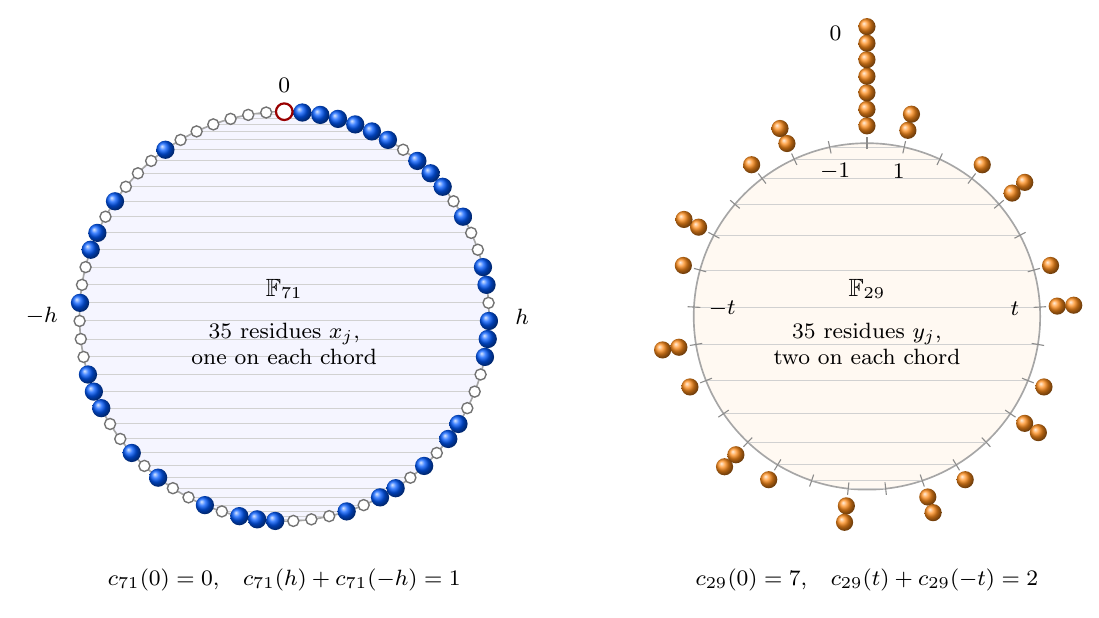
\includegraphics[width=0.98\textwidth]{figures/fig_distributions.png}
\caption{Left: the $35$ residues $x_j$ in $\F_{71}$; each pair $\{h,-h\}$ with $h\ne0$ carries exactly one of them (Lemma~\ref{lem:71}). Right: the residues $y_j$ in $\F_{29}$ in case~(c) of Lemma~\ref{lem:29}; $0$ carries seven of them and each pair $\{t,-t\}$ with $t\ne0$ carries two. Each picture alone is compatible with the projected identity~\eqref{eq:groupring} (Remark~\ref{rem:xz}).}
\label{fig:distributions}
\end{figure}

\subsection{Case (a)}
By Lemma~\ref{lem:p2} with $p=29$, $6m=12354\equiv580\pmod{841}$ would be congruent to $f_{35}(1+2c_{29}(0))$. But $f_{35}(13)=13\cdot14\cdot15-210\cdot13=0$ and $f_{35}(71)=71\,(72\cdot73-210)=6\cdot71\cdot841\equiv0$. Since $580\not\equiv0\pmod{841}$, case~(a) is impossible.

\subsection{The joint projection}\label{ssec:joint}
In cases (b) and (c) we have $c_{29}(t)+c_{29}(-t)=D$ for every $t\ne0$, with $D=1$ and $c_{29}(0)=21$, or $D=2$ and $c_{29}(0)=7$. Let $\Gamma=\F_{71}\times\F_{29}$ and $\psi=(\psi_1,\psi_2)\colon G\to\Gamma$. The image of $\psi$ is a subgroup of the cyclic group $\Gamma$ of order $2059$ whose order is divisible by $71$ and by $29$, because both projections are onto; so $\psi$ is surjective and $|G|/|\Gamma|=29$.

Let $R_0=\F_{71}[\F_{29}]$ and let $\Lambda=R_0[\varepsilon]/(\varepsilon^2)$ be the ring of dual numbers over $R_0$. The map
\[
\chi(s,t)=\gp{t}\,(1+s\varepsilon)=\gp{t}+s\gp{t}\,\varepsilon,\qquad (s,t)\in\Gamma,
\]
is a homomorphism $\Gamma\to\Lambda^\times$, because $(1+s\varepsilon)(1+s'\varepsilon)=1+(s+s')\varepsilon$. The left side of~\eqref{eq:chi} is
\[
6\cdot29\sum_{t\in\F_{29}}\gp{t}\Bigl(71+\Bigl(\sum_{s\in\F_{71}}s\Bigr)\varepsilon\Bigr)=0,
\]
because $71=0$ and $\sum_{s\in\F_{71}}s=71\cdot35=0$ in $\F_{71}$. On the right side $T_i=U_i+N_i\varepsilon$ with
\[
U_i=\gp0+\sum_j\bigl(\gp{iy_j}+\gp{-iy_j}\bigr),\qquad N_i=i\sum_jx_j\bigl(\gp{iy_j}-\gp{-iy_j}\bigr)\qquad\text{in }R_0.
\]
Taking the coefficient of $\varepsilon$ in~\eqref{eq:chi} gives
\begin{equation}\label{eq:eps}
3U_1^2N_1+3(U_1N_2+U_2N_1)+2N_3-6nN_1=0.
\end{equation}
The coefficient of $U_i$ at $t$ is $\delta_{t,0}+c_{29}(i^{-1}t)+c_{29}(-i^{-1}t)$, which equals $1+2c_{29}(0)$ at $t=0$ and $D$ at $t\ne0$. Hence $U_i=A\gp0+DS$ with $S=S_{\F_{29}}$ and $A=1+2c_{29}(0)-D$. Since $S\gp{t}=S$ for every $t$, we get $SN_i=0$, and~\eqref{eq:eps} becomes
\begin{equation}\label{eq:epsA}
(3A^2+3A-6n)N_1+3AN_2+2N_3=0.
\end{equation}
For $t\in\F_{29}$ put
\[
s(t)=\sum_{j:\,y_j=t}x_j-\sum_{j:\,y_j=-t}x_j\in\F_{71}.
\]
The coefficient of $N_i$ at $t$ is $i\,s(i^{-1}t)$. In $\F_{29}$ we have $2^{-1}=15$ and $3^{-1}=10$, so~\eqref{eq:epsA} says that
\begin{equation}\label{eq:rel}
(3A^2+3A-6n)\,s(t)+6A\,s(15t)+6\,s(10t)=0\qquad\text{for every }t\in\F_{29}.
\end{equation}
In case~(b), $A=42$, and the coefficients are $5208\equiv25$, $252\equiv39$ and $6$ modulo $71$. In case~(c), $A=13$, and they are $336\equiv52$, $78\equiv7$ and $6$. Multiplying by $12=6^{-1}$ in $\F_{71}$, we obtain
\begin{equation}\label{eq:relab}
a\,s(t)+b\,s(15t)+s(10t)=0\qquad\text{for every }t\in\F_{29},
\end{equation}
with $(a,b)=(16,42)$ in case~(b) and $(a,b)=(56,13)$ in case~(c).

\subsection{A circulant system}\label{ssec:circ}
The residue $2$ is a primitive root modulo $29$: $2^4=16\ne1$, $2^7=128\equiv12$ and $2^{14}\equiv144\equiv-1$, so the order of $2$ divides $28$ but not $14$ or $4$. Hence $15=2^{-1}$ has order $28$, $15^{14}=-1$, and $15^5=2^{-5}=3^{-1}=10$, since $2^5=32\equiv3$. Put $\mu_k=s(15^k)$ for $k\in\Z$. Then $\mu_{k+28}=\mu_k$, and since $s(-t)=-s(t)$, also $\mu_{k+14}=-\mu_k$. Taking $t=15^k$ in~\eqref{eq:relab} gives
\begin{equation}\label{eq:mu}
a\mu_k+b\mu_{k+1}+\mu_{k+5}=0\qquad\text{for every }k.
\end{equation}
Figure~\ref{fig:orbit} shows these relations on the orbit of $1$.

\begin{figure}[ht]
\centering
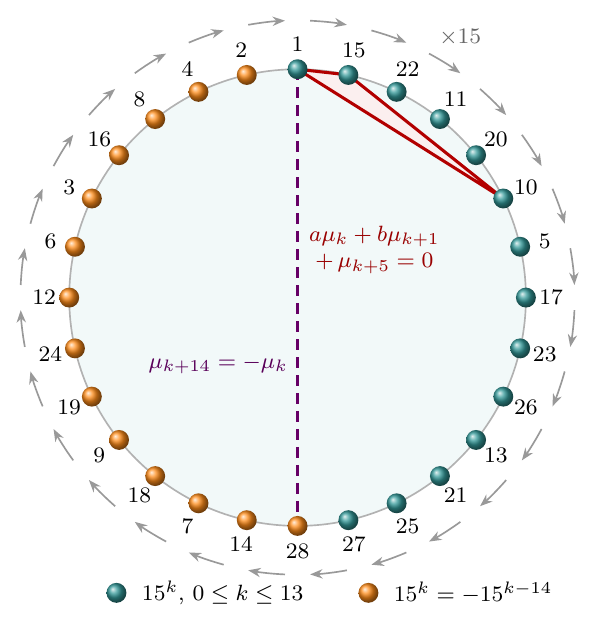
\includegraphics[width=0.56\textwidth]{figures/fig_orbit.png}
\caption{The cyclic group $\F_{29}^\times$ as the orbit $15^k$, $0\le k\le27$. Each relation~\eqref{eq:mu} joins the values of $s$ at $15^k$, $15^{k+1}=2^{-1}\cdot15^k$ and $15^{k+5}=3^{-1}\cdot15^k$ (one instance drawn), and opposite points $15^k$ and $15^{k+14}=-15^k$ carry opposite values of $s$.}
\label{fig:orbit}
\end{figure}

Let $V$ be the $\F_{71}$-vector space of sequences $(\mu_k)_{k\in\Z}$ of period $28$, and let $\sigma$ be the shift, $(\sigma\mu)_k=\mu_{k+1}$. It is invertible, with $\sigma^{-1}=\sigma^{27}$. For our $\mu$ the set $I$ of polynomials $Q\in\F_{71}[X]$ with $Q(\sigma)\mu=0$ is an ideal. It contains $Q=X^5+bX+a$ by~\eqref{eq:mu}, and $X^{14}+1$. Applying $\sigma^5\mu=-(a+b\sigma)\mu$ three times gives $\sigma^{15}\mu=-(a+b\sigma)^3\mu$, while $\sigma^{15}\mu=\sigma\sigma^{14}\mu=-\sigma\mu$. So $I$ also contains $C=(a+bX)^3-X$. All congruences below are modulo $71$.

In case~(b), $C=35X^3-31X^2+21X-22$ and $I$ contains $\widetilde C=-2C=X^3-9X^2+29X-27$. Division with remainder gives
\[
Q=(X^2+9X-19)\,\widetilde C+21X(X+6),\qquad \widetilde C=(X-15)\,X(X+6)-23(X-5).
\]
Hence $X(X+6)\in I$, and then $X-5\in I$. As $\sigma$ is invertible, $(\sigma+6)\mu=0$ and $(\sigma-5)\mu=0$; subtracting, $11\mu=0$, so $\mu=0$.

In case~(c), $C=-4X^3-8X^2-30X+33$ and $I$ contains $\widetilde C=-18C=X^3+2X^2-28X-26$. Here
\[
Q=(X^2-2X+32)\,\widetilde C-23(X-14)^2,\qquad \widetilde C=(X+30)(X-14)^2-23(X+16).
\]
Hence $(X-14)^2\in I$, and then $X+16\in I$. So $\sigma\mu=-16\mu$, and $0=(\sigma-14)^2\mu=30^2\mu=48\mu$; again $\mu=0$.

\subsection{End of the proof}
\begin{proof}[Proof of Theorem~\ref{thm:main} for $n=35$]
Cases (a), (b) and (c) of Lemma~\ref{lem:29} exhaust the possibilities. Case~(a) is impossible, and in cases (b) and (c) we have shown that $\mu=0$, in particular $s(1)=\mu_0=0$. The set $J=\{j:\ y_j=\pm1\}$ has $c_{29}(1)+c_{29}(-1)=D$ elements, and $s(1)=\sum_{j\in J}\pm x_j$. If $D=1$, then $s(1)=\pm x_j$ for one $j$, which is nonzero by Lemma~\ref{lem:71}. If $D=2$, then $s(1)=\pm x_j\pm x_k$ with $j\ne k$, which is nonzero because $x_j\ne\pm x_k$ by Lemma~\ref{lem:71}. Either way $s(1)\ne0$, a contradiction.
\end{proof}

\begin{remark}\label{rem:xz}
Case~(b) can also be excluded without the prime $71$. In cases (b) and (c) the element $T_i$ of~\eqref{eq:groupring} for $\Gamma=\F_{29}$ is $A\gp0+DS$ with integer coefficients, and $S^2=29S$, so the right side of~\eqref{eq:groupring} is $f_{35}(A)\gp0$ plus an integer multiple of $S$. Comparing the coefficients at $\gp0$ and $\gp1$ with those of the left side $6mS$ gives $f_{35}(A)=0$. For $A>0$ this means $(A+1)(A+2)=210$, that is $A=13$, which rules out case~(b), where $A=42$. Case~(c) passes: with $A=13$ and $D=2$ the right side is exactly $12354\,S=6mS$. Likewise the distribution of Lemma~\ref{lem:71} gives $T_i=S_{\F_{71}}$ and a right side $5046\,S_{\F_{71}}=6\cdot841\,S_{\F_{71}}$, as required. So each of the two distributions of Figure~\ref{fig:distributions} satisfies the projected identity~\eqref{eq:groupring} exactly, as Xiao and Zhou observed \cite[Example~5.14]{XZ}, and only the joint projection of Section~\ref{ssec:joint} sees that they cannot occur together.
\end{remark}

\section{Formal verification}\label{sec:lean}

Theorem~\ref{thm:main} has been formalized in Lean~4~\cite{Lean} with the Mathlib library~\cite{Mathlib}. The formal statement defines a lattice tiling of $\Z^n$ by $B^n(r)$ as a subgroup $L$ of $\Z^n$ such that every $x\in\Z^n$ has exactly one $l\in L$ with $\sum_j|x_j-l_j|\le r$, and it asserts that no such subgroup exists for $(n,r)=(35,3)$ or $(805,3)$. The proof follows Sections~\ref{sec:codes}--\ref{sec:35}. Lemma~\ref{lem:reduction}, Proposition~\ref{prop:ball} for an arbitrary commutative ring, Lemmas~\ref{lem:uniform} and~\ref{lem:surj}, Proposition~\ref{prop:moment}, Lemmas~\ref{lem:powersums} and~\ref{lem:counts}, Lemma~\ref{lem:p2} for $p=29$, and the arguments of Sections~\ref{sec:805} and~\ref{sec:35} are proved there, and the finite computations in $\F_{29}$, $\F_{71}$ and $\Z/841$, among them Table~\ref{tab:kappa}, are checked by the kernel. Two steps are argued differently there: the left side of~\eqref{eq:chi} in Section~\ref{ssec:joint} is shown to vanish by pairing each element $x$ of a fibre of $\psi_2$ with $2x_0-x$ for a fixed $x_0$ in that fibre, and the system~\eqref{eq:mu} is solved by an explicit linear combination of its twenty-eight equations. Both theorems depend only on the standard axioms of Lean, namely propositional extensionality, choice and quotient soundness. The numbers in Sections~\ref{sec:805} and~\ref{sec:35} were also recomputed independently by the programs archived with the formalization~\cite{archive}.

\subsection*{Data and code availability}
\begingroup\raggedright
The \LaTeX{} source of the paper, the Lean~4 formalisation of Theorem~\ref{thm:main} described in Section~\ref{sec:lean}, and the C, C\texttt{++}, Python, Julia and shell programs that recompute the finite quantities of Sections~\ref{sec:805} and~\ref{sec:35} are archived at Zenodo under doi:\href{https://doi.org/\zenodoID}{\zenodoID} \cite{archive}; the paper is available at \url{\preprintURL}. Deep Bhattacharjee carried out the computations and the Lean, Julia, C, C\texttt{++}, Python and shell verifications, and the proofs and the text were drafted, with AI assistance (Claude, Anthropic); both authors approved the final version.\par
\endgroup

\subsection*{Ethical declarations}
Funding: none. Competing interests: none.

\begin{thebibliography}{99}
\raggedright

\bibitem{Bha22}
D.~Bhattacharjee, \emph{Establishing equivariant class $[O]$ for hyperbolic groups}, Asian Res. J. Math. \textbf{18} (2022), no.~11, 362--369, doi:\href{https://doi.org/10.9734/arjom/2022/v18i11615}{10.9734/arjom/2022/v18i11615}.

\bibitem{archive}
D.~Bhattacharjee and U.~Bhattacharya, \emph{No lattice tiling of $\mathbb{Z}^{35}$ or $\mathbb{Z}^{805}$ by Lee balls of radius three: Lean formalization and programs}, Zenodo, 2026, doi:\href{https://doi.org/\zenodoID}{\zenodoID}.

\bibitem{BBB26a}
D.~Bhattacharjee, U.~Bhattacharya and S.~Bhattacharya, \emph{The sphere packing problem in dimension $4$}, Preprints.org, 2026.\newline doi:\href{https://doi.org/10.20944/preprints202606.0856.v11}{10.20944/preprints202606.0856.v11}.

\bibitem{BBB26b}
D.~Bhattacharjee, U.~Bhattacharya and S.~Bhattacharya, \emph{The sphere packing problem in dimension $7$}, Preprints.org, 2026.\newline doi:\href{https://doi.org/10.20944/preprints202606.1534.v9}{10.20944/preprints202606.1534.v9}.

\bibitem{DF}
R.~Dougherty and V.~Faber, \emph{The degree-diameter problem for several varieties of Cayley graphs~I: the abelian case}, SIAM J. Discrete Math. \textbf{17} (2004), 478--519, doi:\href{https://doi.org/10.1137/S0895480100372899}{10.1137/S0895480100372899}.

\bibitem{GW}
S.~W.~Golomb and L.~R.~Welch, \emph{Perfect codes in the Lee metric and the packing of polyominoes}, SIAM J. Appl. Math. \textbf{18} (1970), 302--317, doi:\href{https://doi.org/10.1137/0118025}{10.1137/0118025}.

\bibitem{GMP}
S.~Gravier, M.~Mollard and C.~Payan, \emph{On the non-existence of $3$-dimensional tiling in the Lee metric}, European J. Combin. \textbf{19} (1998), 567--572, doi:\href{https://doi.org/10.1006/eujc.1998.0211}{10.1006/eujc.1998.0211}.

\bibitem{Hor09}
P.~Horak, \emph{Tilings in Lee metric}, European J. Combin. \textbf{30} (2009), 480--489, doi:\href{https://doi.org/10.1016/j.ejc.2008.04.007}{10.1016/j.ejc.2008.04.007}.

\bibitem{HA}
P.~Horak and B.~F.~AlBdaiwi, \emph{Diameter perfect Lee codes}, IEEE Trans. Inform. Theory \textbf{58} (2012), 5490--5499, doi:\href{https://doi.org/10.1109/TIT.2012.2196257}{10.1109/TIT.2012.2196257}.

\bibitem{HK}
P.~Horak and D.~Kim, \emph{50 years of the Golomb--Welch conjecture}, IEEE Trans. Inform. Theory \textbf{64} (2018), 3048--3061, doi:\href{https://doi.org/10.1109/TIT.2017.2786675}{10.1109/TIT.2017.2786675}.

\bibitem{Kim}
D.~Kim, \emph{Nonexistence of perfect $2$-error-correcting Lee codes in certain dimensions}, European J. Combin. \textbf{63} (2017), 1--5, doi:\href{https://doi.org/10.1016/j.ejc.2017.01.007}{10.1016/j.ejc.2017.01.007}.

\bibitem{Lean}
L.~de~Moura and S.~Ullrich, \emph{The Lean~4 theorem prover and programming language}, in: Automated Deduction -- CADE 28, Lecture Notes in Comput. Sci. 12699, Springer, 2021, pp.~625--635, doi:\href{https://doi.org/10.1007/978-3-030-79876-5_37}{10.1007/978-3-030-79876-5\_37}.

\bibitem{LZ}
K.~H.~Leung and Y.~Zhou, \emph{No lattice tiling of $\mathbb{Z}^n$ by Lee sphere of radius $2$}, J. Combin. Theory Ser. A \textbf{171} (2020), 105157, doi:\href{https://doi.org/10.1016/j.jcta.2019.105157}{10.1016/j.jcta.2019.105157}.

\bibitem{Mathlib}
The mathlib Community, \emph{The Lean mathematical library}, in: Proceedings of the 9th ACM SIGPLAN International Conference on Certified Programs and Proofs (CPP 2020), ACM, 2020, pp.~367--381, doi:\href{https://doi.org/10.1145/3372885.3373824}{10.1145/3372885.3373824}.

\bibitem{Post}
K.~A.~Post, \emph{Nonexistence theorems on perfect Lee codes over large alphabets}, Inform. and Control \textbf{29} (1975), 369--380, doi:\href{https://doi.org/10.1016/S0019-9958(75)80005-2}{10.1016/S0019-9958(75)80005-2}.

\bibitem{Qur}
C.~Qureshi, \emph{On the non-existence of linear perfect Lee codes: the Zhang--Ge condition and a new polynomial criterion}, European J. Combin. \textbf{83} (2020), 103022, doi:\href{https://doi.org/10.1016/j.ejc.2019.103022}{10.1016/j.ejc.2019.103022}.

\bibitem{Sze}
M.~Szegedy, \emph{Algorithms to tile the infinite grid with finite clusters}, in: Proceedings of the 39th Annual Symposium on Foundations of Computer Science (FOCS 1998), IEEE, 1998, pp.~137--145, doi:\href{https://doi.org/10.1109/SFCS.1998.743437}{10.1109/SFCS.1998.743437}.

\bibitem{XZ}
A.~Xiao and Y.~Zhou, \emph{On the lattice tilings by Lee balls: $Q$-polynomials, group-ring equations, and a decision algorithm}, arXiv:\href{https://arxiv.org/abs/2610.19775}{2610.19775}, 2026.

\bibitem{ZG17}
T.~Zhang and G.~Ge, \emph{Perfect and quasi-perfect codes under the $l_p$ metric}, IEEE Trans. Inform. Theory \textbf{63} (2017), 4325--4331, doi:\href{https://doi.org/10.1109/TIT.2017.2685424}{10.1109/TIT.2017.2685424}.

\bibitem{ZG24}
T.~Zhang and G.~Ge, \emph{On linear diameter perfect Lee codes with distance $6$}, J. Combin. Theory Ser. A \textbf{201} (2024), 105816, doi:\href{https://doi.org/10.1016/j.jcta.2023.105816}{10.1016/j.jcta.2023.105816}.

\bibitem{ZZ}
T.~Zhang and Y.~Zhou, \emph{On the nonexistence of lattice tilings of $\mathbb{Z}^n$ by Lee spheres}, J. Combin. Theory Ser. A \textbf{165} (2019), 225--257, doi:\href{https://doi.org/10.1016/j.jcta.2019.02.008}{10.1016/j.jcta.2019.02.008}.

\end{thebibliography}

\end{document}
